\documentclass[10.5pt]{article}
\usepackage[utf8]{inputenc}\usepackage[T1]{fontenc}
\usepackage{amsmath,amsthm,amssymb,enumitem,booktabs,xcolor,tikz,longtable,array,needspace,graphicx}
\usepackage{geometry}
\newcommand{\sect}[1]{\par\medskip\noindent\textbf{\large #1}\par\smallskip}
\theoremstyle{definition}\newtheorem*{example}{Example}\newtheorem*{method*}{Method}
\theoremstyle{remark}\newtheorem*{remark}{Remark}

\newcommand{\chili}{\tikz[baseline=-0.25ex,scale=0.5]{\fill[red!80!black](0,0.12)..controls(0.3,0.16)and(0.55,0.0)..(0.66,-0.22)..controls(0.42,-0.07)and(0.2,-0.04)..(0,-0.1)--cycle;\fill[green!45!black](-0.04,-0.02)rectangle(0.04,0.16);}}
\newcommand{\spice}[1]{\foreach\i in {1,...,#1}{\chili\,}}
\geometry{letterpaper,margin=0.8in}\setlength{\parindent}{0pt}\setlength{\parskip}{0.3em}

\begin{document}

{\Large\textbf{Slot 14 key: the table as a map of configurations}}\par

\sect{When each module is used}\begin{itemize}[itemsep=1pt,leftmargin=1.4em]
\item \textbf{Review (L1 to L4), 0:00--6:00.} On the board as students sit down; they work alone, notes face down.
\item \textbf{Concept C1 to C3} are the three live questions (whiteboards, sample two): C1 at 13:00, C2 at 17:00, C3 at 18:30. C4 to C6 are on the sheet.
\item \textbf{Practice, 26:00--41:00.} The core is C4 to C6 and P1 to P5 (14.0 minutes). P6 to P9 are the bank: finishers or homework.
\item \textbf{Challenge H1 to H4} are for students who finish the core; students write what they tried before asking for a nudge.
\end{itemize}

\textit{Spice: \spice{1} one step, \spice{2} two steps or an explanation, \spice{3} a graph, two steps or an argument, \spice{4} a hidden quantity.}\par

\begin{center}
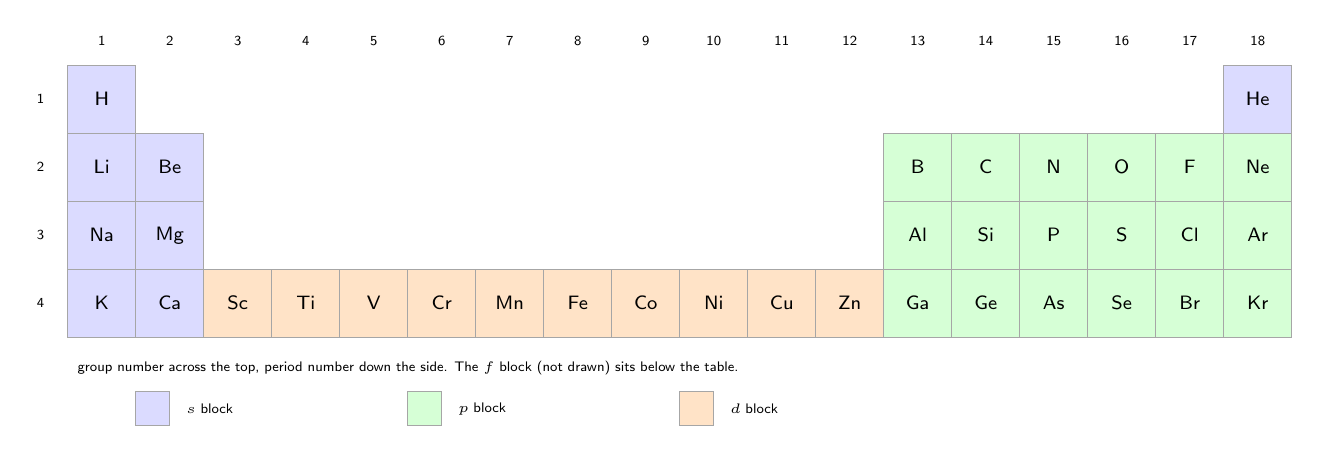
\begin{tikzpicture}[x=0.34in,y=-0.34in,every node/.style={font=\scriptsize\sffamily}]
\node[font=\tiny\sffamily] at (0.50,-0.35) {1};
\node[font=\tiny\sffamily] at (1.50,-0.35) {2};
\node[font=\tiny\sffamily] at (2.50,-0.35) {3};
\node[font=\tiny\sffamily] at (3.50,-0.35) {4};
\node[font=\tiny\sffamily] at (4.50,-0.35) {5};
\node[font=\tiny\sffamily] at (5.50,-0.35) {6};
\node[font=\tiny\sffamily] at (6.50,-0.35) {7};
\node[font=\tiny\sffamily] at (7.50,-0.35) {8};
\node[font=\tiny\sffamily] at (8.50,-0.35) {9};
\node[font=\tiny\sffamily] at (9.50,-0.35) {10};
\node[font=\tiny\sffamily] at (10.50,-0.35) {11};
\node[font=\tiny\sffamily] at (11.50,-0.35) {12};
\node[font=\tiny\sffamily] at (12.50,-0.35) {13};
\node[font=\tiny\sffamily] at (13.50,-0.35) {14};
\node[font=\tiny\sffamily] at (14.50,-0.35) {15};
\node[font=\tiny\sffamily] at (15.50,-0.35) {16};
\node[font=\tiny\sffamily] at (16.50,-0.35) {17};
\node[font=\tiny\sffamily] at (17.50,-0.35) {18};
\node[font=\tiny\sffamily] at (-0.4,0.50) {1};
\node[font=\tiny\sffamily] at (-0.4,1.50) {2};
\node[font=\tiny\sffamily] at (-0.4,2.50) {3};
\node[font=\tiny\sffamily] at (-0.4,3.50) {4};
\fill[blue!14] (0,0) rectangle (1,1);\draw[gray!70,line width=0.3pt] (0,0) rectangle (1,1);
\node at (0.50,0.50) {H};
\fill[blue!14] (17,0) rectangle (18,1);\draw[gray!70,line width=0.3pt] (17,0) rectangle (18,1);
\node at (17.50,0.50) {He};
\fill[blue!14] (0,1) rectangle (1,2);\draw[gray!70,line width=0.3pt] (0,1) rectangle (1,2);
\node at (0.50,1.50) {Li};
\fill[blue!14] (1,1) rectangle (2,2);\draw[gray!70,line width=0.3pt] (1,1) rectangle (2,2);
\node at (1.50,1.50) {Be};
\fill[green!16] (12,1) rectangle (13,2);\draw[gray!70,line width=0.3pt] (12,1) rectangle (13,2);
\node at (12.50,1.50) {B};
\fill[green!16] (13,1) rectangle (14,2);\draw[gray!70,line width=0.3pt] (13,1) rectangle (14,2);
\node at (13.50,1.50) {C};
\fill[green!16] (14,1) rectangle (15,2);\draw[gray!70,line width=0.3pt] (14,1) rectangle (15,2);
\node at (14.50,1.50) {N};
\fill[green!16] (15,1) rectangle (16,2);\draw[gray!70,line width=0.3pt] (15,1) rectangle (16,2);
\node at (15.50,1.50) {O};
\fill[green!16] (16,1) rectangle (17,2);\draw[gray!70,line width=0.3pt] (16,1) rectangle (17,2);
\node at (16.50,1.50) {F};
\fill[green!16] (17,1) rectangle (18,2);\draw[gray!70,line width=0.3pt] (17,1) rectangle (18,2);
\node at (17.50,1.50) {Ne};
\fill[blue!14] (0,2) rectangle (1,3);\draw[gray!70,line width=0.3pt] (0,2) rectangle (1,3);
\node at (0.50,2.50) {Na};
\fill[blue!14] (1,2) rectangle (2,3);\draw[gray!70,line width=0.3pt] (1,2) rectangle (2,3);
\node at (1.50,2.50) {Mg};
\fill[green!16] (12,2) rectangle (13,3);\draw[gray!70,line width=0.3pt] (12,2) rectangle (13,3);
\node at (12.50,2.50) {Al};
\fill[green!16] (13,2) rectangle (14,3);\draw[gray!70,line width=0.3pt] (13,2) rectangle (14,3);
\node at (13.50,2.50) {Si};
\fill[green!16] (14,2) rectangle (15,3);\draw[gray!70,line width=0.3pt] (14,2) rectangle (15,3);
\node at (14.50,2.50) {P};
\fill[green!16] (15,2) rectangle (16,3);\draw[gray!70,line width=0.3pt] (15,2) rectangle (16,3);
\node at (15.50,2.50) {S};
\fill[green!16] (16,2) rectangle (17,3);\draw[gray!70,line width=0.3pt] (16,2) rectangle (17,3);
\node at (16.50,2.50) {Cl};
\fill[green!16] (17,2) rectangle (18,3);\draw[gray!70,line width=0.3pt] (17,2) rectangle (18,3);
\node at (17.50,2.50) {Ar};
\fill[blue!14] (0,3) rectangle (1,4);\draw[gray!70,line width=0.3pt] (0,3) rectangle (1,4);
\node at (0.50,3.50) {K};
\fill[blue!14] (1,3) rectangle (2,4);\draw[gray!70,line width=0.3pt] (1,3) rectangle (2,4);
\node at (1.50,3.50) {Ca};
\fill[orange!22] (2,3) rectangle (3,4);\draw[gray!70,line width=0.3pt] (2,3) rectangle (3,4);
\node at (2.50,3.50) {Sc};
\fill[orange!22] (3,3) rectangle (4,4);\draw[gray!70,line width=0.3pt] (3,3) rectangle (4,4);
\node at (3.50,3.50) {Ti};
\fill[orange!22] (4,3) rectangle (5,4);\draw[gray!70,line width=0.3pt] (4,3) rectangle (5,4);
\node at (4.50,3.50) {V};
\fill[orange!22] (5,3) rectangle (6,4);\draw[gray!70,line width=0.3pt] (5,3) rectangle (6,4);
\node at (5.50,3.50) {Cr};
\fill[orange!22] (6,3) rectangle (7,4);\draw[gray!70,line width=0.3pt] (6,3) rectangle (7,4);
\node at (6.50,3.50) {Mn};
\fill[orange!22] (7,3) rectangle (8,4);\draw[gray!70,line width=0.3pt] (7,3) rectangle (8,4);
\node at (7.50,3.50) {Fe};
\fill[orange!22] (8,3) rectangle (9,4);\draw[gray!70,line width=0.3pt] (8,3) rectangle (9,4);
\node at (8.50,3.50) {Co};
\fill[orange!22] (9,3) rectangle (10,4);\draw[gray!70,line width=0.3pt] (9,3) rectangle (10,4);
\node at (9.50,3.50) {Ni};
\fill[orange!22] (10,3) rectangle (11,4);\draw[gray!70,line width=0.3pt] (10,3) rectangle (11,4);
\node at (10.50,3.50) {Cu};
\fill[orange!22] (11,3) rectangle (12,4);\draw[gray!70,line width=0.3pt] (11,3) rectangle (12,4);
\node at (11.50,3.50) {Zn};
\fill[green!16] (12,3) rectangle (13,4);\draw[gray!70,line width=0.3pt] (12,3) rectangle (13,4);
\node at (12.50,3.50) {Ga};
\fill[green!16] (13,3) rectangle (14,4);\draw[gray!70,line width=0.3pt] (13,3) rectangle (14,4);
\node at (13.50,3.50) {Ge};
\fill[green!16] (14,3) rectangle (15,4);\draw[gray!70,line width=0.3pt] (14,3) rectangle (15,4);
\node at (14.50,3.50) {As};
\fill[green!16] (15,3) rectangle (16,4);\draw[gray!70,line width=0.3pt] (15,3) rectangle (16,4);
\node at (15.50,3.50) {Se};
\fill[green!16] (16,3) rectangle (17,4);\draw[gray!70,line width=0.3pt] (16,3) rectangle (17,4);
\node at (16.50,3.50) {Br};
\fill[green!16] (17,3) rectangle (18,4);\draw[gray!70,line width=0.3pt] (17,3) rectangle (18,4);
\node at (17.50,3.50) {Kr};
\node[font=\tiny\sffamily,anchor=west] at (0,4.45) {group number across the top, period number down the side. The $f$ block (not drawn) sits below the table.};
\fill[blue!14] (1,4.8) rectangle (1.5,5.3);\draw[gray!70,line width=0.3pt] (1,4.8) rectangle (1.5,5.3);\node[anchor=west,font=\tiny\sffamily] at (1.6,5.05) {$s$ block};
\fill[green!16] (5,4.8) rectangle (5.5,5.3);\draw[gray!70,line width=0.3pt] (5,4.8) rectangle (5.5,5.3);\node[anchor=west,font=\tiny\sffamily] at (5.6,5.05) {$p$ block};
\fill[orange!22] (9,4.8) rectangle (9.5,5.3);\draw[gray!70,line width=0.3pt] (9,4.8) rectangle (9.5,5.3);\node[anchor=west,font=\tiny\sffamily] at (9.6,5.05) {$d$ block};
\end{tikzpicture}
\end{center}

\sect{Review (L1 to L4)}

\noindent\hangindent=7em\hangafter=1\makebox[7em][l]{\textbf{L1}}Write the full configuration of lithium (Z = 3).\par\noindent\hspace{7em}\textbf{Answer.} $1s^{2}2s^{1}$.\par\smallskip

\noindent\hangindent=7em\hangafter=1\makebox[7em][l]{\textbf{L2}}Write the full configuration of sodium (Z = 11).\par\noindent\hspace{7em}\textbf{Answer.} $1s^{2}2s^{2}2p^{6}3s^{1}$.\par\smallskip

\noindent\hangindent=7em\hangafter=1\makebox[7em][l]{\textbf{L3}}Lithium and sodium are in the same group. What do the last pieces of their configurations have in common?\par\noindent\hspace{7em}\textbf{Answer.} Both end in $s^{1}$: one electron in the outer shell. This is the slot 13 pattern (group 1) showing up as a configuration.\par\smallskip

\noindent\hangindent=7em\hangafter=1\makebox[7em][l]{\textbf{L4}}Guess, no penalty: how many elements are in the fourth row of the periodic table?\par\noindent\hspace{7em}\textbf{Answer.} The answer is 18. Do not say so yet. Come back to the guess at 13:00 (live C1) and ask who was close.\par\smallskip

\sect{Conceptual questions}

\needspace{4\baselineskip}\noindent\hangindent=7em\hangafter=1\makebox[7em][l]{\textbf{C1}\ \spice{2}}Period 3 has 8 elements and period 4 has 18. What does period 4 have that period 3 does not?\par\noindent\hangindent=7em\hangafter=0\hspace{7em}\textbf{Answer.} The $3d$ subshell: ten more boxes between $4s$ and $4p$. Check the L4 guess (18).\par\noindent\hspace{7em}\textit{Likely error: Period 4 has 8 elements like the others.}\par\medskip

\needspace{4\baselineskip}\noindent\hangindent=7em\hangafter=1\makebox[7em][l]{\textbf{C2}\ \spice{1}}Which block are potassium, iron and gallium in?\par\noindent\hangindent=7em\hangafter=0\hspace{7em}\textbf{Answer.} K is $s$, Fe is $d$, Ga is $p$.\par\noindent\hspace{7em}\textit{Likely error: The $d$ block starts at shell 3.}\par\medskip

\needspace{4\baselineskip}\noindent\hangindent=7em\hangafter=1\makebox[7em][l]{\textbf{C3}\ \spice{2}}Chlorine is in group 17. Write its valence configuration and count its valence electrons.\par\noindent\hangindent=7em\hangafter=0\hspace{7em}\textbf{Answer.} $3s^{2}3p^{5}$, 7 valence electrons.\par\medskip

\needspace{4\baselineskip}\noindent\hangindent=7em\hangafter=1\makebox[7em][l]{\textbf{C4}\ \spice{2}}Think and rank. Without looking at the table, rank these atoms from the fewest valence electrons to the most: (A) chlorine, (B) magnesium, (C) aluminum, (D) argon. Then check on the table.\par\noindent\hangindent=7em\hangafter=0\hspace{7em}\textbf{Answer.} B, C, A, D: magnesium 2, aluminum 3, chlorine 7, argon 8.\par\noindent\hspace{7em}\textit{Likely error: Ranking by atomic number (12, 13, 17, 18) happens to give the same order here. Ask: would it for sodium and neon? No: neon (8) has more valence electrons than sodium (1) but a lower Z than sodium.}\par\medskip

\needspace{4\baselineskip}\noindent\hangindent=7em\hangafter=1\makebox[7em][l]{\textbf{C5}\ \spice{2}}A student says: ``Every atom in group 18 has 8 valence electrons.'' When is that true, and when is it not?\par\noindent\hangindent=7em\hangafter=0\hspace{7em}\textbf{Answer.} True for neon, argon and krypton ($g-10=8$). Not true for helium: it has only the $1s$ subshell, so 2 valence electrons.\par\noindent\hspace{7em}\textit{Likely error: Group 18 means 8 for helium. It has only the 1s subshell.}\par\medskip

\needspace{4\baselineskip}\noindent\hangindent=7em\hangafter=1\makebox[7em][l]{\textbf{C6}\ \spice{2}}A student writes: ``Arsenic is in period 4, group 15, so it is $4s^{2}3d^{3}$.'' Find the error and fix it.\par\noindent\hangindent=7em\hangafter=0\hspace{7em}\textbf{Answer.} Group 15 is in the $p$ block (groups 13--18), not the $d$ block (groups 3--12). Arsenic is $4s^{2}4p^{3}$, with 5 valence electrons.\par\noindent\hspace{7em}\textit{Likely error: The d block is groups 3--12 only.}\par\medskip

\sect{Practice}

\needspace{4\baselineskip}\noindent\hangindent=7em\hangafter=1\makebox[7em][l]{\textbf{P1}\ \spice{1}}On the table above, shade the $s$ block, the $p$ block and the $d$ block with three different patterns. Write the period number beside each row. Mark with an arrow where the $f$ block would sit.\par\noindent\hangindent=7em\hangafter=0\hspace{7em}\textbf{Answer.} Groups 1--2 shaded $s$ (He also sits in group 18 but is an $s$-element); groups 13--18 shaded $p$; groups 3--12 shaded $d$ (period 4 only). Periods 1 to 4 down the side. The $f$ block is named only: it sits below the table.\par\medskip

\needspace{4\baselineskip}\noindent\hangindent=7em\hangafter=1\makebox[7em][l]{\textbf{P2}\ \spice{1}}Give the block, period and group of (a) magnesium (Z = 12), (b) chlorine (Z = 17), (c) iron (Z = 26). Read them off the table.\par\noindent\hangindent=7em\hangafter=0\hspace{7em}\textbf{Answer.} (a) s block, period 3, group 2. (b) p block, period 3, group 17. (c) d block, period 4, group 8.\par\medskip

\needspace{4\baselineskip}\noindent\hangindent=7em\hangafter=1\makebox[7em][l]{\textbf{P3}\ \spice{1}}Write the valence configuration, with no full configuration, for the element in (a) period 2, group 2; (b) period 3, group 13; (c) period 3, group 15.\par\noindent\hangindent=7em\hangafter=0\hspace{7em}\textbf{Answer.} (a) $2s^{2}$. (b) $3s^{2}3p^{1}$. (c) $3s^{2}3p^{3}$.\par\medskip

\needspace{4\baselineskip}\noindent\hangindent=7em\hangafter=1\makebox[7em][l]{\textbf{P4}\ \spice{2}}Which element has the valence configuration (a) $3s^{1}$? (b) $4s^{2}4p^{2}$? Give its period and group.\par\noindent\hangindent=7em\hangafter=0\hspace{7em}\textbf{Answer.} (a) Na, period 3, group 1. (b) Ge, period 4, group 14.\par\medskip

\needspace{4\baselineskip}\noindent\hangindent=7em\hangafter=1\makebox[7em][l]{\textbf{P5}\ \spice{2}}An atom's full configuration is $1s^{2}2s^{2}2p^{6}3s^{2}3p^{6}4s^{2}3d^{8}$. Add up the electrons to find Z, then give the element, block, period and group.\par\noindent\hangindent=7em\hangafter=0\hspace{7em}\textbf{Answer.} $2+2+6+2+6+2+8 = 28$: nickel, d block, period 4, group 10. The last subshell filled is $3d$, so it is a $d$-block atom, and its period is the highest shell, 4.\par\noindent\hspace{7em}\textit{Likely error: Students stop at 3d and call nickel period 3. The period is the highest shell number (4), not 3. ASK: what is the highest shell number?}\par\medskip

\needspace{4\baselineskip}\noindent\hangindent=7em\hangafter=1\makebox[7em][l]{\textbf{P6}\ \spice{2}}Give the block, period and group of (a) potassium (Z = 19), (b) gallium (Z = 31), (c) krypton (Z = 36). Then write the valence configuration of (b) and (c).\par\noindent\hangindent=7em\hangafter=0\hspace{7em}\textbf{Answer.} (a) s block, period 4, group 1. (b) p block, period 4, group 13; valence $4s^{2}4p^{1}$. (c) p block, period 4, group 18; valence $4s^{2}4p^{6}$, 8 valence electrons.\par\noindent\hspace{7em}\textit{Likely error: Gallium has 3d10 filled, but 3d is not in the outer shell. Valence means the outer shell: 4s and 4p only.}\par\medskip

\needspace{4\baselineskip}\noindent\hangindent=7em\hangafter=1\makebox[7em][l]{\textbf{P7}\ \spice{1}}Which element has the valence configuration (a) $2s^{2}2p^{4}$? (b) $4s^{2}4p^{5}$? How many valence electrons does each have?\par\noindent\hangindent=7em\hangafter=0\hspace{7em}\textbf{Answer.} (a) O, 6. (b) Br, 7.\par\medskip

\needspace{4\baselineskip}\noindent\hangindent=7em\hangafter=1\makebox[7em][l]{\textbf{P8}\ \spice{2}}An element is in period 4, the $d$ block, group 7. Name it and give its atomic number.\par\noindent\hangindent=7em\hangafter=0\hspace{7em}\textbf{Answer.} Manganese, Z = 25. Its full configuration ends $4s^{2}3d^{5}$.\par\noindent\hspace{7em}\textit{Likely error: Period 4, not period 3: the 3d subshell fills after 4s.}\par\medskip

\needspace{4\baselineskip}\noindent\hangindent=7em\hangafter=1\makebox[7em][l]{\textbf{P9}\ \spice{2}}Which element in period 3 has 3 valence electrons? Which has 5? Which has 7?\par\noindent\hangindent=7em\hangafter=0\hspace{7em}\textbf{Answer.} Al, P and Cl.\par\medskip

\sect{Challenge}

\needspace{4\baselineskip}\noindent\hangindent=7em\hangafter=1\makebox[7em][l]{\textbf{H1}\ \spice{3}}The graph shows the number of valence electrons for every atom from $Z=3$ to $Z=18$.\par\medskip
\begin{center}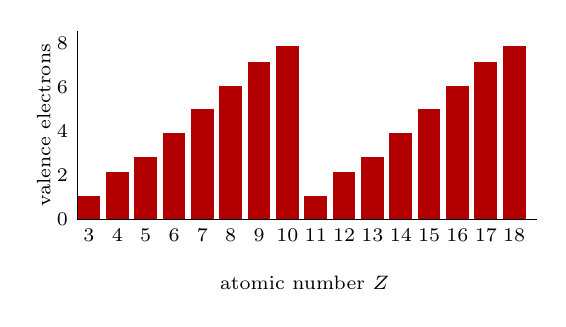
\begin{tikzpicture}[x=0.36cm]\fill[red!70!black] (0,0) rectangle (0.8,0.3);\fill[red!70!black] (1,0) rectangle (1.8,0.6);\fill[red!70!black] (2,0) rectangle (2.8,0.8);\fill[red!70!black] (3,0) rectangle (3.8,1.1);\fill[red!70!black] (4,0) rectangle (4.8,1.4);\fill[red!70!black] (5,0) rectangle (5.8,1.7);\fill[red!70!black] (6,0) rectangle (6.8,2.0);\fill[red!70!black] (7,0) rectangle (7.8,2.2);\fill[red!70!black] (8,0) rectangle (8.8,0.3);\fill[red!70!black] (9,0) rectangle (9.8,0.6);\fill[red!70!black] (10,0) rectangle (10.8,0.8);\fill[red!70!black] (11,0) rectangle (11.8,1.1);\fill[red!70!black] (12,0) rectangle (12.8,1.4);\fill[red!70!black] (13,0) rectangle (13.8,1.7);\fill[red!70!black] (14,0) rectangle (14.8,2.0);\fill[red!70!black] (15,0) rectangle (15.8,2.2);\draw (0,0)--(16.2,0);\draw (0,0)--(0,2.4);\node[font=\scriptsize,below] at (0.4,0){3};\node[font=\scriptsize,below] at (1.4,0){4};\node[font=\scriptsize,below] at (2.4,0){5};\node[font=\scriptsize,below] at (3.4,0){6};\node[font=\scriptsize,below] at (4.4,0){7};\node[font=\scriptsize,below] at (5.4,0){8};\node[font=\scriptsize,below] at (6.4,0){9};\node[font=\scriptsize,below] at (7.4,0){10};\node[font=\scriptsize,below] at (8.4,0){11};\node[font=\scriptsize,below] at (9.4,0){12};\node[font=\scriptsize,below] at (10.4,0){13};\node[font=\scriptsize,below] at (11.4,0){14};\node[font=\scriptsize,below] at (12.4,0){15};\node[font=\scriptsize,below] at (13.4,0){16};\node[font=\scriptsize,below] at (14.4,0){17};\node[font=\scriptsize,below] at (15.4,0){18};\node[font=\scriptsize,left] at (0,0.00){0};\node[font=\scriptsize,left] at (0,0.56){2};\node[font=\scriptsize,left] at (0,1.12){4};\node[font=\scriptsize,left] at (0,1.68){6};\node[font=\scriptsize,left] at (0,2.24){8};\node[font=\scriptsize] at (8,-0.8){atomic number $Z$};\node[font=\scriptsize,rotate=90] at (-1.2,1.2){valence electrons};\end{tikzpicture}\end{center}(a) At which $Z$ does the graph reach 8, each time? (b) At which $Z$ does it fall back to 1? (c) How many elements are between those two falls? Say what that number means about the shell. (d) Predict the next $Z$ where the graph would show 1, and name the element.\par\noindent\hangindent=7em\hangafter=0\hspace{7em}\textbf{Answer.} (a) $Z=10$ and $Z=18$ (neon and argon). (b) $Z=3$ and $Z=11$ (lithium and sodium). (c) 8 elements, $Z=3$ to $10$: that is the $s$ and $p$ boxes of one shell (2 + 6). (d) $Z=19$, potassium: period 4, group 1, $4s^{1}$.\par\noindent\hspace{7em}\textit{Likely error: Students say the next 1 is at $Z=19$ and stop. Ask: what else fills before the next $p$ block? (the 3d, ten more elements, but they are not on this graph).}\par\medskip

\needspace{4\baselineskip}\noindent\hangindent=7em\hangafter=1\makebox[7em][l]{\textbf{H2}\ \spice{3}}An atom has 34 electrons. Use the filling order to write its full configuration, then give its period, block, group, valence configuration and number of valence electrons.\par\noindent\hangindent=7em\hangafter=0\hspace{7em}\textbf{Answer.} Full: $1s^{2}2s^{2}2p^{6}3s^{2}3p^{6}4s^{2}3d^{10}4p^{4}$. The last subshell filled is $4p$, so $p$ block, period 4, group $4p^{4}\to 12+4=16$. Selenium (Se), valence $4s^{2}4p^{4}$, 6 valence electrons. Check: $16-10=6$.\par\noindent\hspace{7em}\textit{Likely error: Counting $3d^{10}$ as valence (16 valence electrons), or calling it period 3.}\par\medskip

\needspace{4\baselineskip}\noindent\hangindent=7em\hangafter=1\makebox[7em][l]{\textbf{H3}\ \spice{3}}A student says: ``Chlorine is in group 17, so it has 17 valence electrons.'' Write a reply, in two or three sentences, that corrects the claim and tells the student how to get the right number from the table.\par\noindent\hangindent=7em\hangafter=0\hspace{7em}\textbf{Answer.} Group 17 is the 17th column, not the electron count. Chlorine is in period 3, the $p$ block; its valence configuration is $3s^{2}3p^{5}$, so it has 7 valence electrons ($g-10=7$). The first ten columns are not counted because the $d$ block (groups 3--12) sits between group 2 and group 13.\par\noindent\hspace{7em}\textit{Likely error: Reply says only ``it is 7'' with no reason. A full reply gives the number and the rule.}\par\medskip

\needspace{4\baselineskip}\noindent\hangindent=7em\hangafter=1\makebox[7em][l]{\textbf{H4}\ \spice{4}}Suppose the filling order were $1s,\ 2s,\ 2p,\ 3s,\ 3p,\ 3d,\ 4s,\ 4p$ (the $3d$ before $4s$). Start a new row each time the outer shell number goes up. How many elements would each of the four rows hold? Explain in one sentence why the real table has rows of 2, 8, 8 and 18 instead.\par\noindent\hangindent=7em\hangafter=0\hspace{7em}\textbf{Answer.} Rows of 2, 8, 18 and 8. Real order: $4s$ fills before $3d$, so the $3d$ boxes land in shell 4. Because the row number is the highest shell filled, those ten boxes go in period 4.\par\noindent\hspace{7em}\textit{Likely error: Students rebuild the real order and answer 2, 8, 8, 18. Ask: which subshell did you put third in the list?}\par\medskip

\sect{Hint ladders (spice 3 and 4, one rung at a time, after the student shows what was tried)}\begin{description}[leftmargin=2.2em,itemsep=2pt]

\item[H1] (1) Look at the heights first. Which $Z$ values reach the tallest bar, and which sit at the shortest?\ (2) Each fall back to 1 starts a new row of the table. Count the bars from one fall to the next.\ (3) The two falls are at $Z=3$ and $Z=11$. The gap between them is $11-3=$ ?. Then add that gap to 11 and check against the ladder.

\item[H2] (1) Fill the subshells in the ladder order and keep a running total of electrons.\ (2) Stop at 34 total. The last subshell you filled names the block, and the highest shell number is the period.\ (3) Running total: $1s$ 2, $2s$ 4, $2p$ 10, $3s$ 12, $3p$ 18, $4s$ 20, $3d$ 30. Four electrons are left for $4p$.

\item[H3] (1) Where does the student get the number 17? What does that number actually count?\ (2) Which block is group 17 in, and which subshells does it fill in its own shell?\ (3) Write the valence configuration of chlorine, count the electrons, then say why the group number and the electron count differ by 10.

\item[H4] (1) Count boxes in each subshell: $s$ is 2 electrons, $p$ is 6, $d$ is 10. Then list which subshells belong to which shell number.\ (2) In the new order, shell 3 owns $3s$, $3p$ and $3d$ before shell 4 starts. Add them up.\ (3) Row 1: $2$. Row 2: $2+6=8$. Row 3: $2+6+10=$ ? Row 4: $2+6=$ ?. The total must be 36. Then compare with the real rows, 2, 8, 8, 18.

\end{description}

\sect{Exit slip scale (3 points)}\begin{tabular}{@{}lc@{}}\toprule Row & Points\\\midrule
Position marked at the right period and group & 1\\
The right block shaded & 1\\
Valence configuration and valence count written, matching the position & 1\\\bottomrule\end{tabular}\par
Answer for the slip: period 3, group 14 is silicon, $p$ block, $3s^{2}3p^{2}$, 4 valence electrons.

\sect{Sim swap-in}No sim replaces this day: the table is the object. (Checked in code: every configuration, position, valence count, the C4 ranking, the H1 graph values and the H4 row sizes; the clock sums to 50; the core is 14.0 of 15 minutes.)

\par\smallskip{\footnotesize Problems are original, modeled on the style of Hewitt's Conceptual Physics Think and Rank and standard chemistry textbook practice sets.}

\end{document}